\section{Packet Analysis}
\begin{enumerate}[a.]
    \item We ran a DNS filter on the output to {\tt iitd.ac.in} and got the following result(\cref{fig:IITDDNS}):
    \begin{figure}[!ht]
        \centering
        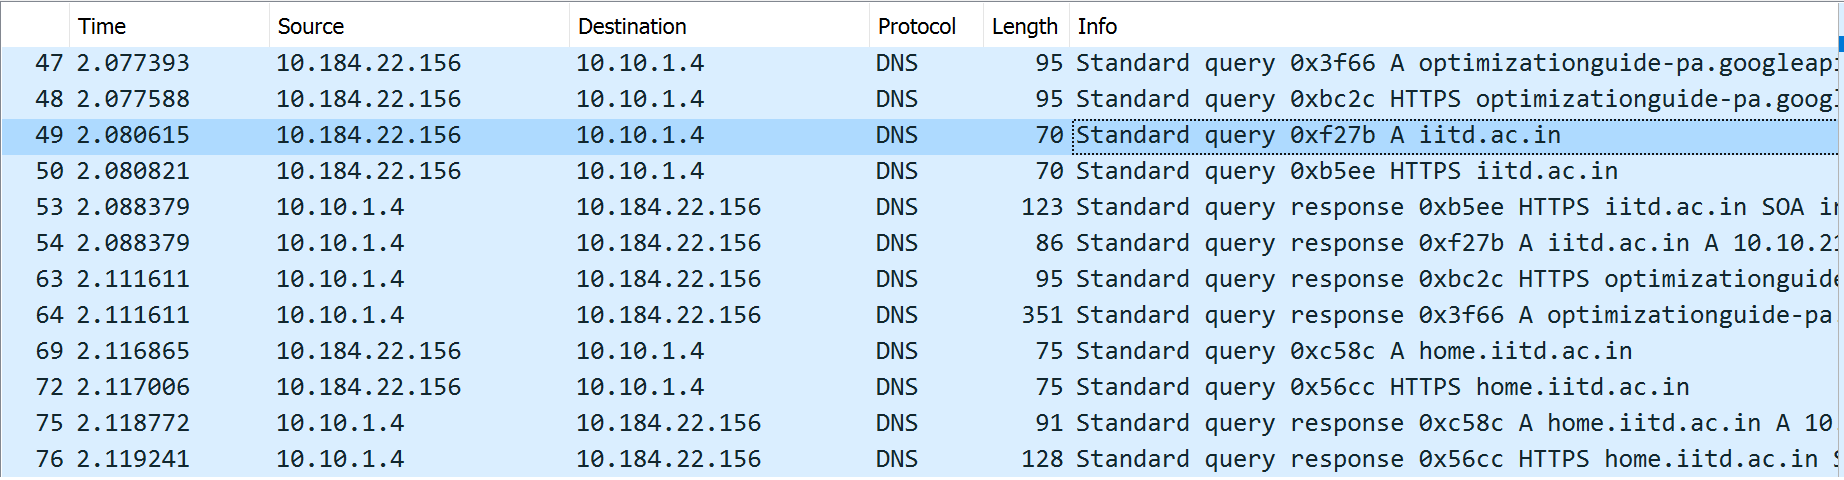
\includegraphics[scale=0.5]{images/IITD dns.png}
        \caption{IITD DNS}
        \label{fig:IITDDNS}
    \end{figure}
    \subsection*{Observations}
    There was 1 DNS query and response for {\tt iitd.ac.in}. The request-response began at 2.080615s and ended at 2.088379s lasting for a total of 7.764ms.
    
    \item On applying a {\tt http} filter, only one request is observed as shown in \cref{fig:IITDHTTP}
    \begin{figure}[!ht]
        \centering
        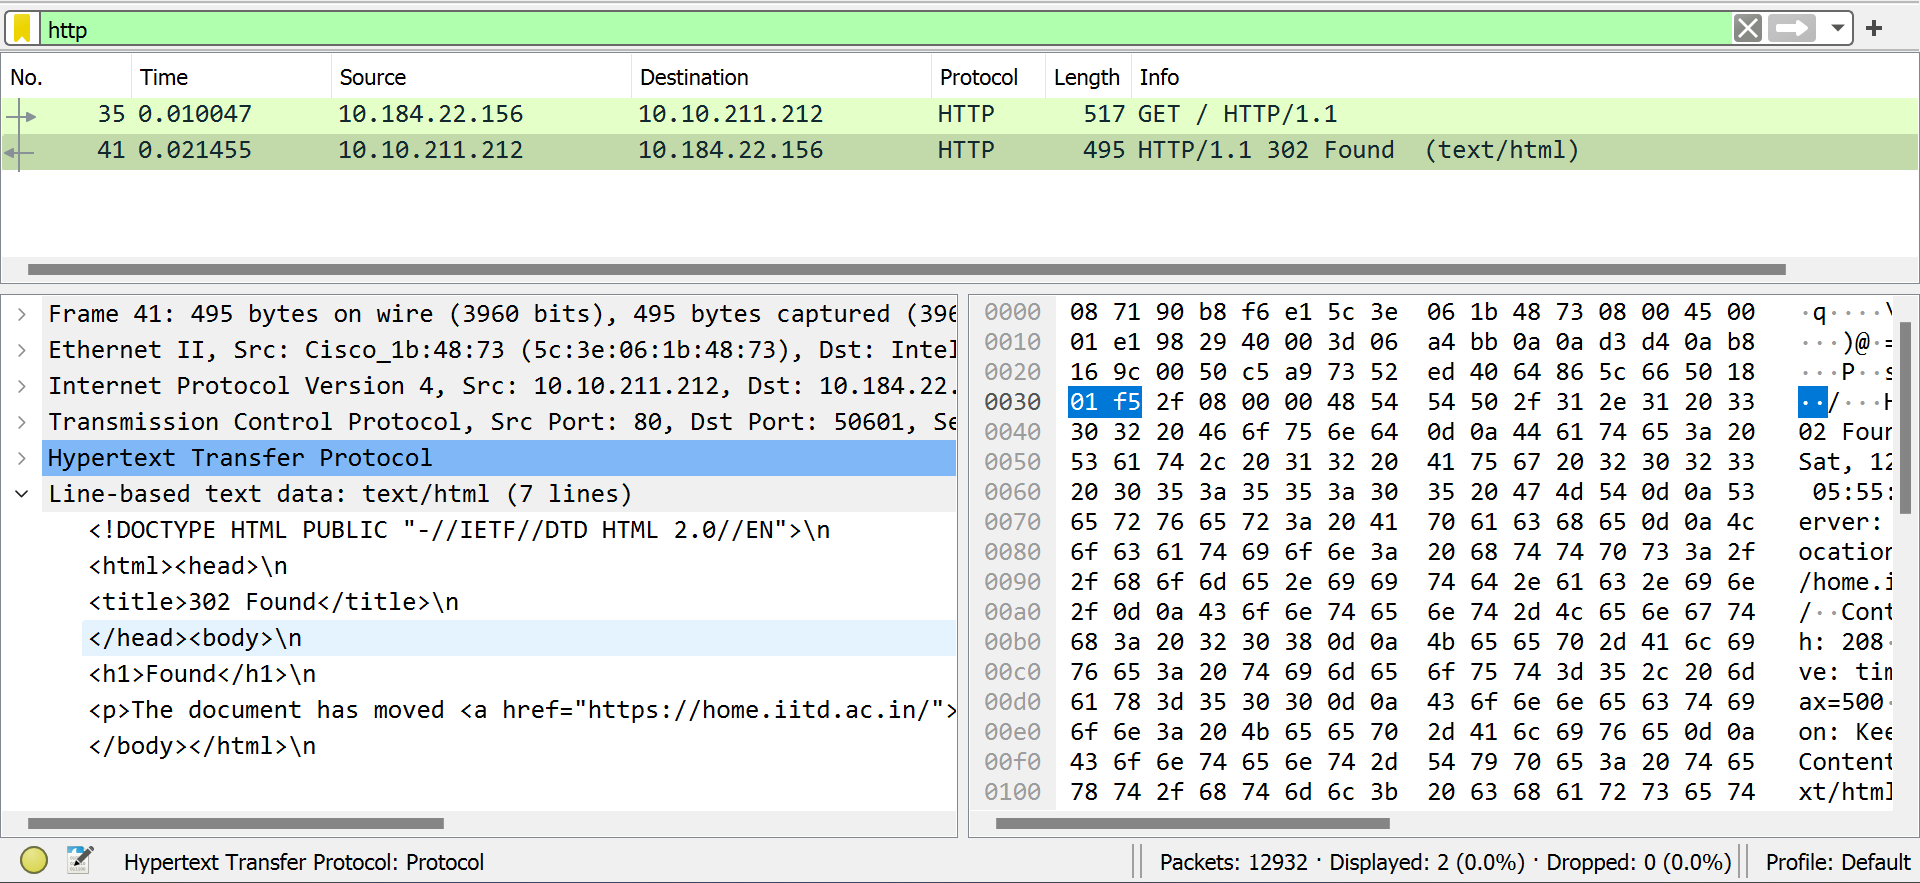
\includegraphics[scale=0.5]{images/IITD http.png}
        \caption{IITD HTTP}
        \label{fig:IITDHTTP}
    \end{figure}
    \subsection*{Observations}
    Only one request is observed. The request was for {\tt http://www.iitd.ac.in/} and the response was {\tt 302 Found} indicating that the requested resource has been moved to a different URL. The text data tells us that "The document has moved {\tt https://home.iitd.ac.in/}".

    HTTPS traffic is encrypted using SSL/TLS, and the contents of the packets are scrambled and unreadable without the decryption keys. Hence, we are not able to find any html / css / js files for the webpage in the packets.

    
    \item Next we applied the filter {\tt ((ip.src==10.184.22.156 \&\& ip.dst==10.10.211.212) || (ip.src==10.10.211.212 \&\& ip.dst==10.184.22.156)) \&\& tcp} to get the TCP packets between the two hosts. The output is shown in \cref{fig:IITDTCP}
    \begin{figure}[!ht]
        \centering
        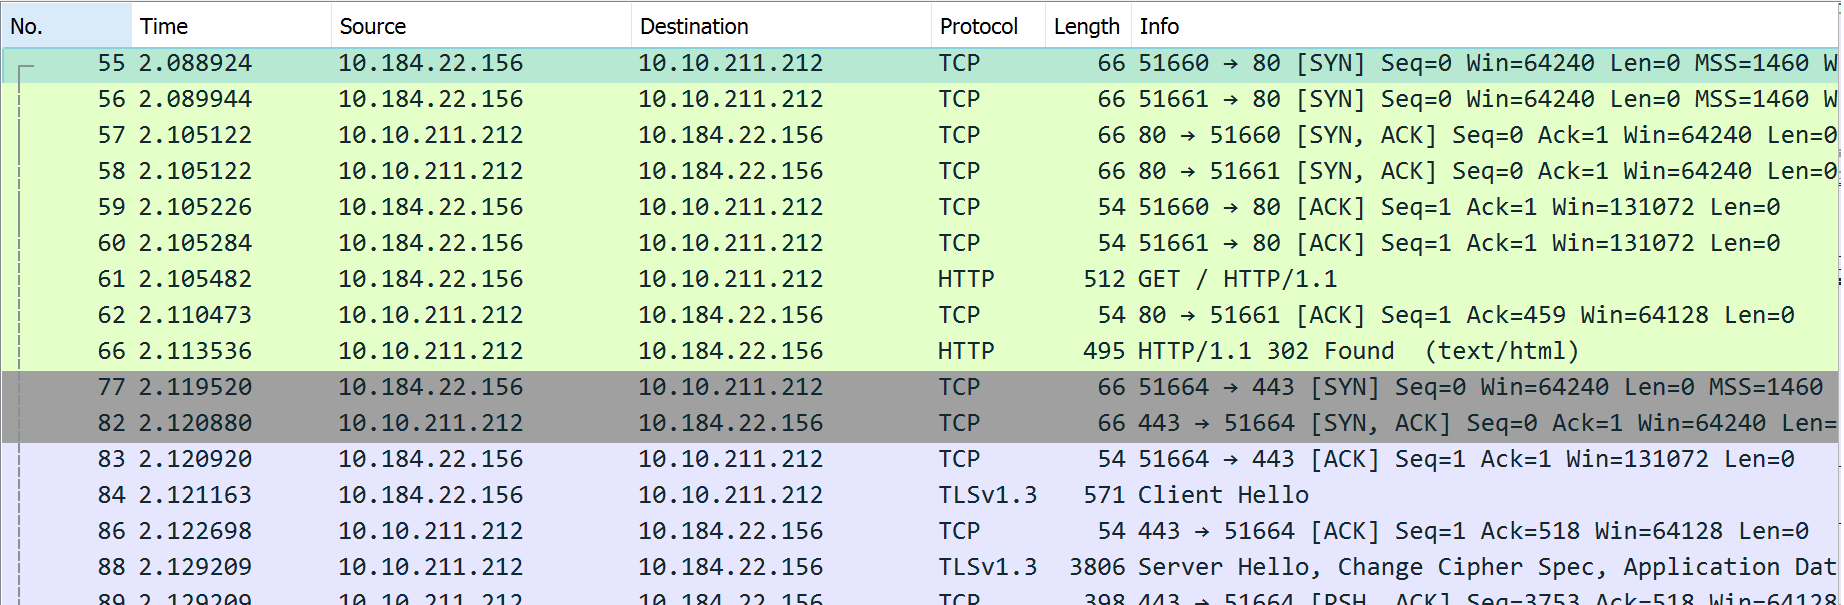
\includegraphics[scale=0.5]{images/IITD tcp.png}
        \caption{IITD TCP}
        \label{fig:IITDTCP}
    \end{figure}
    \subsection*{Observations}
    Total 9 connections were opened. Of these 2 were {\tt http} and 7 were {\tt https}, as identified by their port number (80 for {\tt http} and 443 for {\tt https}). Thus, for the {\tt http} request in part (b), we have 2 corresponding tcp connections. 
    % 57, 58, 82, 316, 317, 332, 333, 339, 2134    

    \item On running a {\tt http} filter on {\tt indianexpress.com}, we received the output \cref{fig:IndianExpress}
    \begin{figure}[!ht]
        \centering
        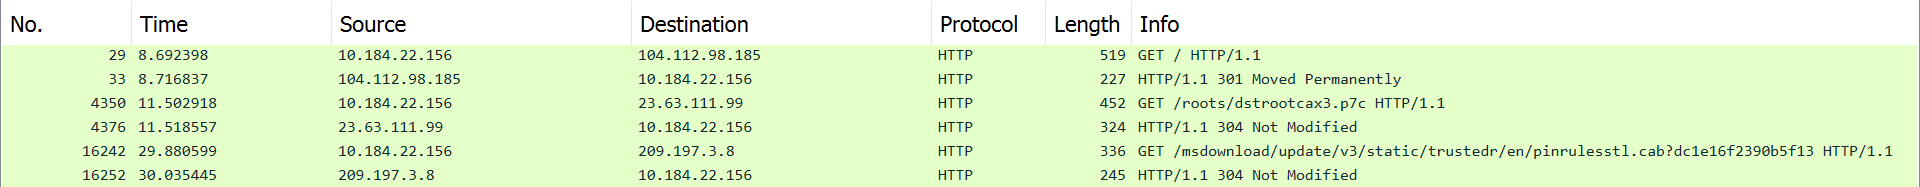
\includegraphics[scale=0.5]{images/indianexpress.png}
        \caption{Indian Express}
        \label{fig:IndianExpress}
    \end{figure}
    \subsection*{Observations}
    As mentioned above, HTTPS traffic is encrypted using SSL/TLS, and the contents of the packets are unreadable without the decryption keys. Hence, we see a very sparse http traffic and are not able to find any html/css/js files being transferred for the webpage in the packets. Wireshark can capture the encrypted packets, but the payload will appear as encrypted gibberish.
\end{enumerate}

\clearpage

Similarly, we ran the filters for {\tt act4d.iitd.ac.in} and got the outputs \cref{fig:ACT4DDNS} \cref{fig:ACT4DHTTP} \cref{fig:ACT4DTCP}:
\begin{figure}[!ht]
    \centering
    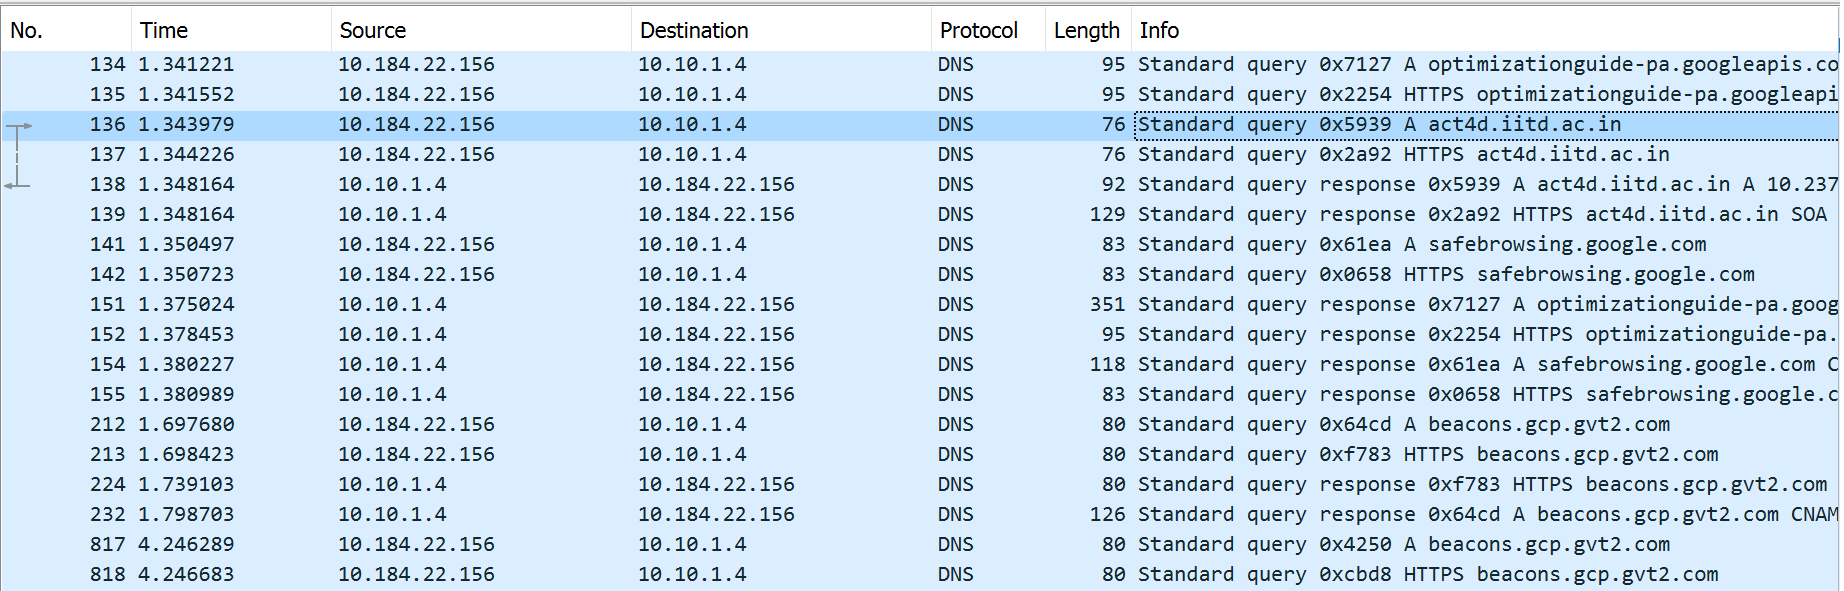
\includegraphics[scale=0.5]{images/act4d dns.png}
    \caption{ACT4D DNS}
    \label{fig:ACT4DDNS}
\end{figure}

\begin{figure}[!ht]
    \centering
    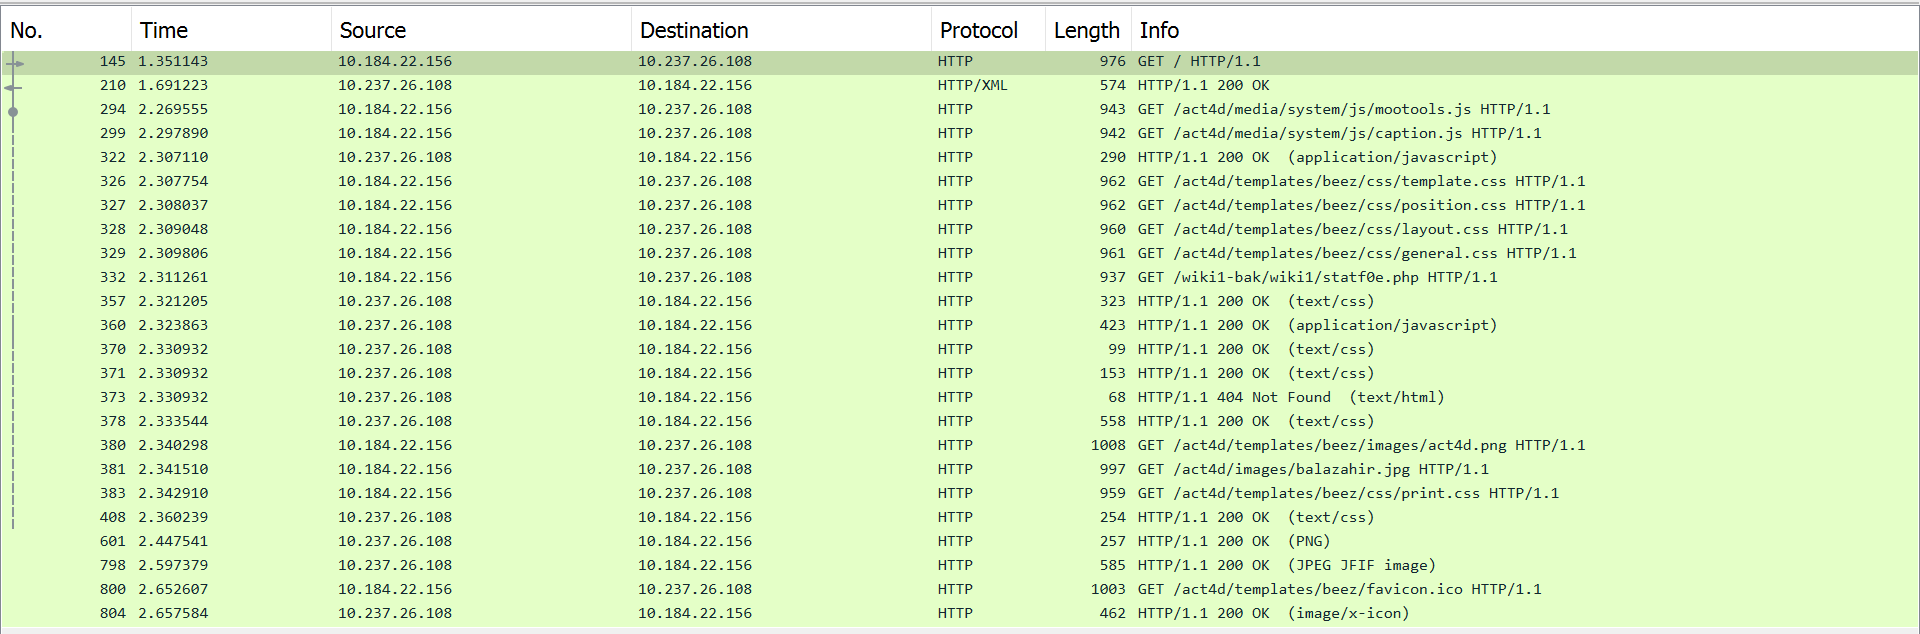
\includegraphics[scale=0.5]{images/act4d http.png}
    \caption{ACT4D http}
    \label{fig:ACT4DHTTP}
\end{figure}

\begin{figure}[!ht]
    \centering
    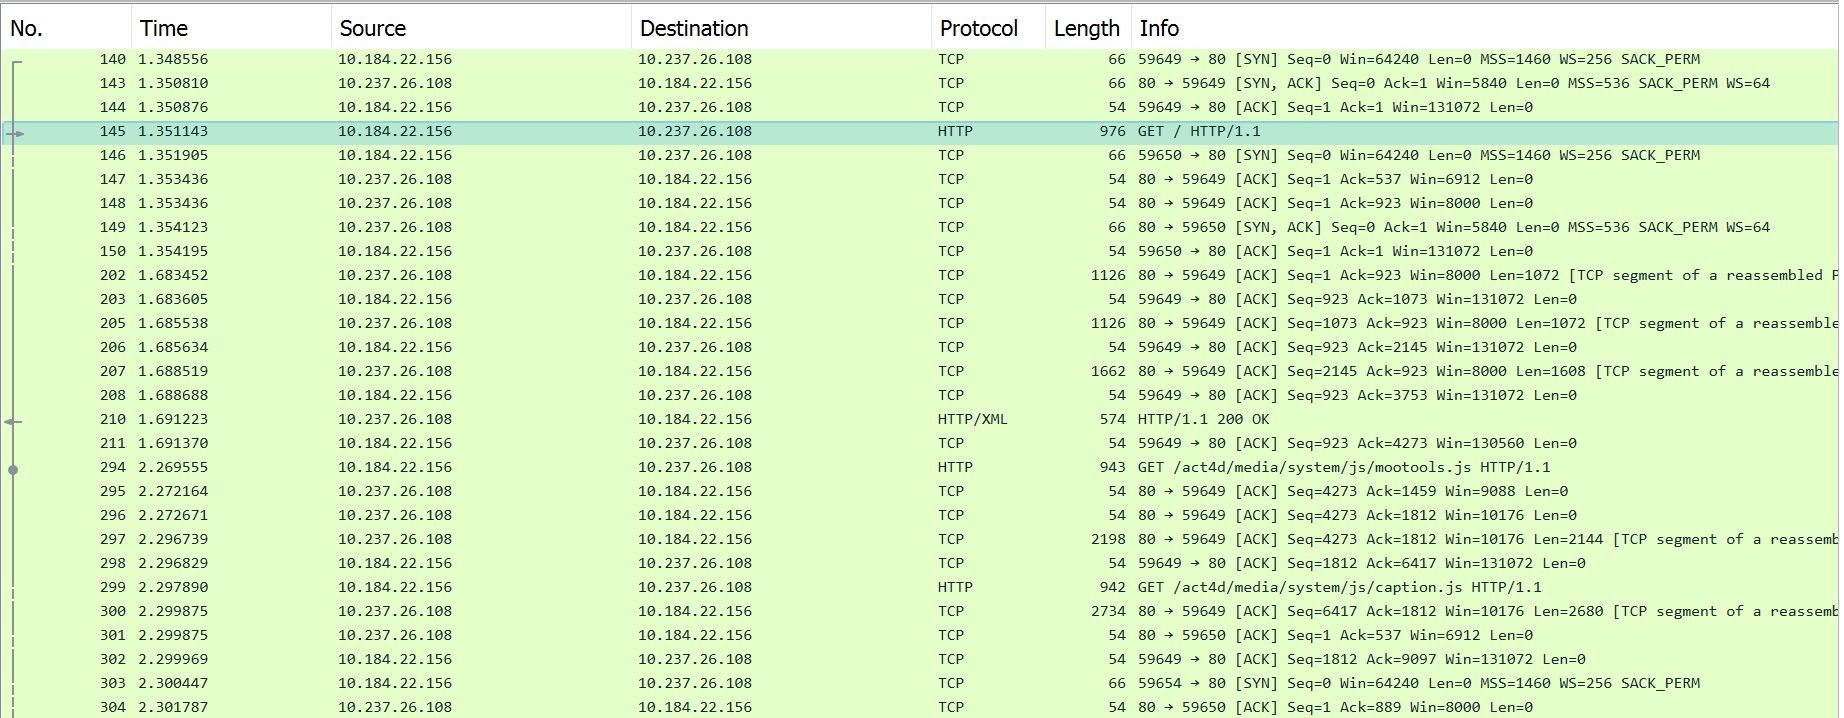
\includegraphics[scale=0.5]{images/act4d tcp.png}
    \caption{ACT4D TCP (filter {\tt ((ip.src==10.184.22.156 \&\& ip.dst==10.237.26.108) || 
    (ip.src==10.237.26.108 \&\& ip.dst==10.184.22.156)) \&\& tcp})}
    \label{fig:ACT4DTCP}
\end{figure}

\subsection*{Observations}
\begin{enumerate}[a. ]
    \item There were DNS queries and responses for {\tt act4d.iitd.ac.in}. The request-response began at 1.343979s and ended at 1.348164s lasting for a total of 4.185ms.
    \item A total of 12 {\tt http} requests were observed. Further, the rough order of requests is as follows:
        \begin{enumerate}
            \item HTML-1
            \item JavaScript-2
            \item CSS-5
            \item PHP-1 (Not found)
            \item Images-3
        \end{enumerate}
        This gives a fair idea about the way a browser loads a webpage. Initially, it prioritizes the loading of the HTML file, which serves as the blueprint for the webpage's structure. Subsequently, it proceeds to fetch JavaScript and CSS files, which respectively provide the interactivity and visual styling essential for the webpage's functionality and aesthetics.

        Concluding this sequence, the browser focuses on loading images. These visual elements, while essential for content enhancement, often possess a larger file size. Hence, deferring their loading until the end optimizes the overall loading performance.

        In essence, this loading hierarchy ensures an organized and efficient rendering process, enabling the browser to progressively construct a fully-fledged and visually appealing webpage.
    \item Total 6 tcp connections were opened, which is more than the number of {\tt http} requests. This is because multiple {\tt http} requests can be served over a single tcp connection. The requests served by the connections are sumarized in \cref{tab:pnr}.
    \begin{table}[!ht]
        \centering
        \begin{tabular}{|l|l|}
        \hline
        \textbf{Source Port} & \textbf{Request Handled}           \\ \hline
        59649                & html, monotools.js                 \\ \hline
        59650                & caption.js, favicon, balazahir.jpg \\ \hline
        59654                & layout.css, act4d.png              \\ \hline
        59655                & position.css, print.css            \\ \hline
        59656                & template.css                       \\ \hline
        59657                & general.css                        \\ \hline
        \end{tabular}
        \caption{Ports and Requests}
        \label{tab:pnr}
        \end{table}
\end{enumerate}
Reusing connections helps to improve performance by saving the time taken to establish a connection. Further, the server can also reuse the same resources for multiple requests, which saves time and bandwidth.